% !TeX TS-program = xelatex

\documentclass{beamer}
%Set the slide theme
%Change to meet your taste
% Madrid, Copenhagen, Berlin, ... works
\usetheme{metropolis}

\usepackage{multicol}

\usepackage{xecolor}
\usepackage{amsmath}
%\usefonttheme[onlymath]{serif} %Change the math font

\usepackage{multirow}
\usepackage{tabularx}
\usepackage{booktabs}
\usepackage[sorting=none,style=ieee]{biblatex}
\addbibresource{references.bib}
\usepackage{xepersian}
\settextfont[Path=fonts/]{Parastoo}

%---------------------------------------------------------------------------------
% Seetings to force Beamer works with Xepersian and RTL typesetting
%-------------------------------------------------------------------------------
%\raggedleft

% For right to left lists (itemize and enumerate)
\makeatletter
\newcommand{\RTList}{\raggedleft\rightskip\@totalleftmargin}
\makeatother
% Correct the bullet for RTL texts
\setbeamertemplate{itemize item}{\scriptsize\raise1.25pt%
 \hbox{\donotcoloroutermaths$\blacktriangleleft$}} 

% To force beamer use numbering in captions
\setbeamertemplate{caption}[numbered]{}% Number float-like environments



%---------------------------------------------------------------------------------
\title{
    زنجیره‌سازی کارکردهای مجازی سرویس شبکه با لحاظ محدودیت منابع مدیریتی
}
\subtitle{مهندسی فناوری اطلاعات - شبکه‌های کامپیوتری}
\author{پرهام الوانی}
\institute{دانشکده مهندسی کامپیوتر و فناوری اطلاعات\\دکتر بهادر بخشی}
\date{پاییز ۱۳۹۷}

\begin{document}
\begin{persian}

%------------------------------------------
% Title frame (0)
%------------------------------------------
\begin{frame}
    \titlepage{}
\end{frame}

% To adjust the paragraphs in RTL
\everypar{\rightskip\rightmargin}
%-------------------------------------------------------------------------------
\begin{frame}{فهرست} % 1
    \begin{itemize}\RTList{}
        \item مقدمه
        \item چالش‌ها
        \item سابقه‌ی کارها
        \item تعریف مساله
        \item چالش‌ها و نوآوری‌های مساله
        \item معیار و نحوه‌ی ارزیابی
        \item فرمول‌بندی
        \item مراجع
    \end{itemize}
\end{frame}
%-------------------------------------------------------------------------------
\begin{frame}{مقدمه} % 2
    \begin{itemize}\RTList{}
        \item عدم انعطاف‌پذیری معماری فعلی شبکه
        \item در مجازی‌سازی کارکرد شبکه با استفاده از مجازی‌سازی منابع، می‌توان کارکردها را بر روی سرورهای استاندارد اجرا کرد
        و بهره‌وری منابع را فزایش داده و هزینه‌های انرژی را کاهش داد.
        \item زنجیره سازی کارکرد سرویس نیز امکان ایجاد زنجیره‌ای از کارکردها را به صورت پویا فراهم می‌کند.
    \end{itemize}
\end{frame}
%-------------------------------------------------------------------------------
\begin{frame}{مقدمه} % 2.5
    \begin{itemize}\RTList{}
        \item با توجه به جداسازی زیرساخت از نرم‌افزار کارکردهای شبکه نیاز به هماهنگی میان آن‌ها ایجاد شده است.
        \item به صورت کلی تفاوت‌هایی که با توجه به فرآیند مجازی‌سازی کارکردهای شبکه ایجاد شده‌اند را  می‌توان
        به ترتیب زیر دسته‌بندی نمود:
        \begin{itemize}\RTList{}
            \item زیرساخت مجازی‌سازی شده
            \item کارکردهای شبکه‌ای مجازی‌سازی شده
            \item سرویس‌های شبکه‌ای
        \end{itemize}
    \end{itemize}
\end{frame}
%-------------------------------------------------------------------------------
\begin{frame}{مقدمه} % 3
    \begin{center}\begin{figure}
        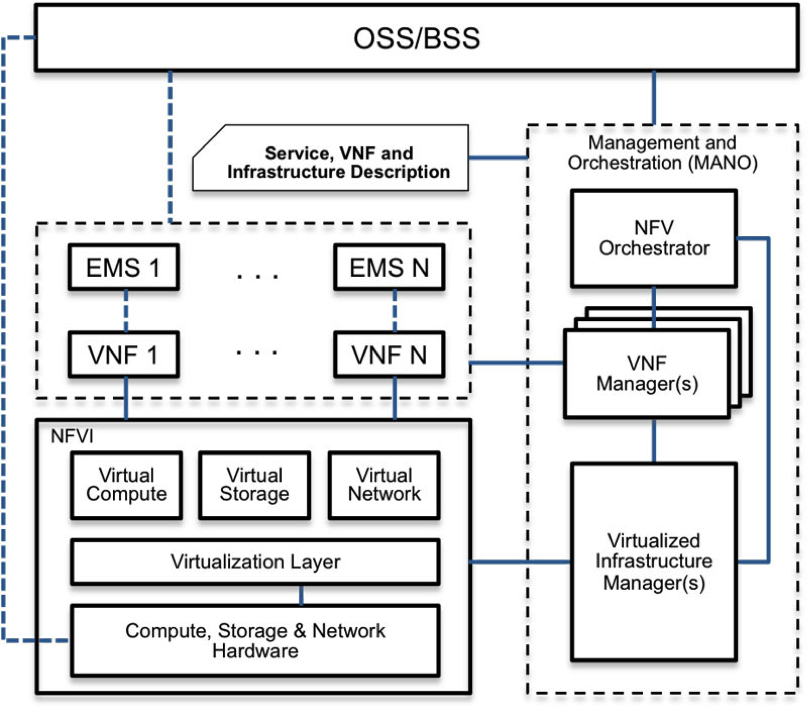
\includegraphics[scale=0.4]{images/nfv-arch.png}
        \caption{معماری سطح بالای مجازی‌سازی کارکردهای شبکه}
    \end{figure}\end{center}
\end{frame}
%-------------------------------------------------------------------------------
\begin{frame}{مقدمه} % 4
    \begin{itemize}\RTList{}
        \item \lr{NFVO} وظیفه‌ی استقرار زنجیره‌های کارکرد سرویس را برعهده دارد.
        \item \lr{VNFM} مسئول چرخه‌ی زندگی کارکردهای مجازی شبکه می‌باشد.
        \item چرخه‌ی زندگی هر کارکرد مجازی شامل عملیات‌هایی همچون نمونه‌سازی، مقیاس‌کردن، به‌روزرسانی و پایان دادن می‌باشد.
        \item هر نمونه از کارکردهای مجازی شبکه نیاز دارد تحت مدیریت یکی از \lr{VNFM}های موحود در شبکه باشد.
    \end{itemize}
\end{frame}
%-------------------------------------------------------------------------------
\begin{frame}{چالش‌ها} % 5
    \begin{columns}
        \begin{column}{0.6\textwidth}
            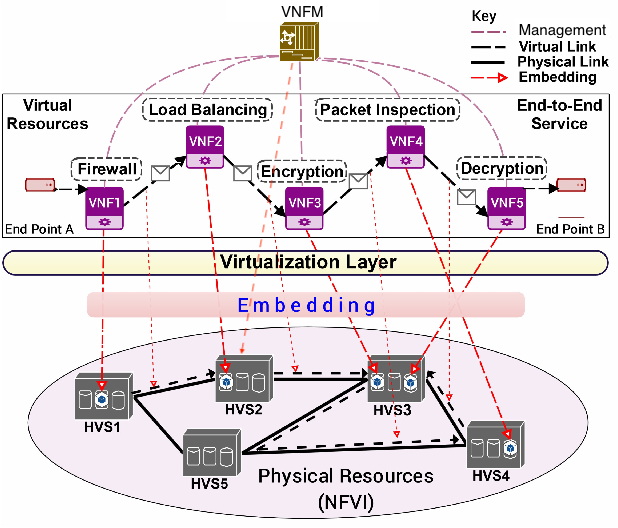
\includegraphics[scale=0.35]{images/embedding.png}
        \end{column}
        \begin{column}{0.4\textwidth}
            \begin{itemize}\RTList{}
                \item مدیریت و هماهنگی
                \item مصرف بهینه‌ی انرژی
                \item تخصیص منابع به کارکردهای مجازی
                \item مسیریابی زنجیره‌های کارکرد سرویس
                \item پذیرش زنجیره‌های کارکرد سرویس
                \item به روزرسانی و مقیاس کردن کارکردهای مجازی سرویس
            \end{itemize}
        \end{column}
    \end{columns}
\end{frame}
%-------------------------------------------------------------------------------
\begin{frame}{سابقه‌ی کارها} % 6
    \fontsize{6pt}{7.2}\selectfont
    \begin{table}[h]
        \caption{مقایسه مقالات پذیرش زنجیره‌های کارکرد سرویس}
        \vspace{0.5cm}
        \begin{tabularx}{\textwidth}{XXXXXXXXXXXXXXXXX}
            \toprule
            منبع &
            \multicolumn{4}{X}{منابع تخصیص یافته} &
            \multicolumn{2}{X}{محدودیت ظرفیت پردازشی نمونه} &
            \multicolumn{2}{X}{برخط یا برون خط} &
            \multicolumn{2}{X}{نگاشت کارکرد و لینک} &
            \multicolumn{2}{X}{انتساب کارکرد} &
            \multicolumn{2}{X}{اشتراک نمونه} &
            \multicolumn{2}{X}{تخصیص \lr{VNFM}} \\
            \midrule
            \lr{\#} &
            \lr{other} &
            \lr{MEM} &
            \lr{BW} &
            \lr{CPU} &
            دارد &
            ندارد &
            برخط &
            برون خط &
            کارکرد &
            لینک &
            یک نمونه &
            چند نمونه &
            دارد &
            ندارد &
            دارد &
            ندارد \\
            \midrule
            \cite{Eramo2016} &
            \lr{---} &
            \lr{---} &
            \checkmark&
            \checkmark&
            \lr{---}&
            \checkmark&
            \lr{---} &
            \checkmark&
            \checkmark&
            \checkmark&
            \checkmark&
            \lr{---} &
            \lr{---} &
            \checkmark&
            \lr{---} &
            \checkmark\\
            \midrule
            \cite{Ghaznavi2017} &
            \lr{---} &
            \lr{---} &
            \checkmark&
            \checkmark&
            \checkmark&
            \lr{---} &
            \lr{---} &
            \checkmark&
            \checkmark&
            \checkmark&
            \lr{---} &
            \checkmark&
            \lr{---} &
            \checkmark&
            \lr{---} &
            \checkmark\\
            \midrule
            \cite{Huang2017} &
            \lr{---} &
            \lr{---} &
            \checkmark&
            \checkmark&
            \checkmark&
            \lr{---} &
            \lr{---} &
            \checkmark&
            \checkmark&
            \checkmark&
            \lr{---} &
            \checkmark&
            \lr{---} &
            \checkmark&
            \lr{---} &
            \checkmark\\
            \midrule
            \cite{AbuLebdeh2017} &
            \lr{VNFM capacity} &
            \lr{---} &
            \lr{---} &
            \lr{---} &
            \lr{---} &
            \checkmark&
            \checkmark&
            \lr{---} &
            \lr{---} &
            \checkmark &
            \lr{---} &
            \lr{---} &
            \lr{---} &
            \lr{---} &
            \checkmark&
            \lr{---} \\
            \midrule
            پژوهش حاضر &
            \lr{---} &
            \checkmark&
            \checkmark&
            \checkmark&
            \checkmark&
            \lr{---} &
            \lr{---} &
            \checkmark&
            \checkmark&
            \checkmark&
            \checkmark&
            \lr{---}&
            \lr{---}&
            \checkmark&
            \checkmark&
            \lr{---}\\
            \bottomrule
        \end{tabularx}
    \end{table}
\end{frame}
%-------------------------------------------------------------------------------
\begin{frame}{سابقه‌ی کارها} % 7
    \begin{itemize}\RTList{}
        \item این مقاله به مانند کار پژوهشی حاضر تاخیر را در لینک‌های مدیریتی در نظر می‌گیرد.
        \item این مقاله فرض می‌کند زنجیره‌ها از پیش پذیرفته شده‌اند.
        \item هدف این مقاله جایگذاری \lr{VNFM}ها به صورت مستقل با هدف کاهش هزینه‌های عملیاتی می‌باشد.
    \end{itemize}
    \begin{latin}
    \fullcite{AbuLebdeh2017}
    \end{latin}
\end{frame}
%-------------------------------------------------------------------------------
\begin{frame}{تعریف مساله} % 8
    \par
    پذیرفتن بیشترین تقاضای زنجیره‌ کارکرد سرویس با در نظر گرفتن نیاز هر نمونه کارکرد مجازی شبکه به یک \lr{VNFM}.
\end{frame}
%-------------------------------------------------------------------------------
\begin{frame}{تعریف مساله} % 9
    \begin{itemize}\RTList{}
        \item توپولوژی زیرساخت شامل پنهای باند لینک‌ها و ظرفیت \lr{NFVI-PoP}ها موجود است.
        \item n تقاضای زنجیره‌ کارکرد سرویس به صورت کامل و از پیش مشخص شده داریم.
        \item هر تقاضا شامل نوع و تعداد نمونه‌های مجازی، پنهای باند لینک‌های مجازی و توپولوژی
        نمونه‌های مجازی می‌باشد.
        \item تعداد پردازنده‌هایی که به هر نمونه تخصیص می‌یابد با توجه به ترافیک ورودی نمونه مشخص می‌شود.
        این امر توسط اپراتور در زمان تعریف مساله صورت می‌پذیرد.
    \end{itemize}
\end{frame}
%-------------------------------------------------------------------------------
\begin{frame}{تعریف مساله} % 10
    \begin{itemize}\RTList{}
        \item نمونه‌ها بین زنجیره‌ها به اشتراک گذاشته نمی‌شوند.
        \item محدودیت ظرفیت لینک‌ها
        \item محدودیت توان پردازش سرورهای فیزیکی با توجه به میزان حافظه و تعداد پردازنده‌ها
    \end{itemize}
\end{frame}
%-------------------------------------------------------------------------------
\begin{frame}{تعریف مساله} % 11
    \begin{itemize}\RTList{}
        \item برای مدیریت یکدست و آسان‌تر زنجیره‌ها و در عین حال جمع‌آوری راحتر خطاها، برای هر زنجیره یک \lr{VNFM} تخصیص می‌دهیم.
        \item \lr{VNFM}ها می‌توانند بین زنجیره به اشتراک گذاشته شوند.
        \item هر نمونه از \lr{VNFM}ها می‌تواند تعداد مشخصی از نمونه‌های کارکرد مجازی شبکه را سرویس دهد. 
        \item برای ارتباط میان هر نمونه از \lr{VNFM}ها و \lr{VNF}ها پهنای باند مشخصی رزرو می‌گردد.
        \item در صورتی که \lr{NFVI-PoP} بتواند از \lr{VNFM} پشتیبانی نماید،
        می‌توان به هر تعداد که ظرفیت آن اجازه می‌دهد بر روی آن \lr{VNFM} نصب نمود.
    \end{itemize}
\end{frame}
%-------------------------------------------------------------------------------
\begin{frame}{چالش‌ها و نوآوری‌های مساله} % 12
    \begin{itemize}\RTList{}
        \item در نظر گرفتن نیازمندی هر نمونه کارکرد مجازی به یک \lr{VNFM}
        \item در نظر گرفتن نیازمندی تاخیر برای لینک‌های مدیریتی
        \item تخصیص منابع مدیریتی به زنجیره‌ها و مسیریابی ارتباط مدیریتی
        \item جایگذاری و مسیریابی توامان زنجیره‌های کارکرد سرویس
    \end{itemize}
\end{frame}
%-------------------------------------------------------------------------------
\begin{frame}{معیار و نحوه‌ی ارزیابی} % 13
    \begin{itemize}\RTList{}
        \item مدل‌سازی مساله
        \item حل مساله‌ی بهینه در ابعاد کوچک
        \item پیاده‌سازی راه‌حل مکاشفه‌ای
        \item معیار مقایسه این راه حل نرخ پذیرش تقاضاهای زنجیره‌های کارکرد سرویس می‌باشد.
        \item مقایسه‌ی نتایج راه‌حل مکاشفه‌ای با جواب بهینه
        \item مقایسه با کارهای مرتبط که نیازمندی‌های مدیریتی را مدنظر قرار نداده‌اند.
    \end{itemize}
\end{frame}
%-------------------------------------------------------------------------------
\begin{frame}{} % 14
    \begin{center}
        فرمول‌بندی و مدل‌سازی ریاضی مساله
    \end{center}
\end{frame}
%-------------------------------------------------------------------------------
\begin{frame}{فرمول‌بندی} % 15
    \par پارامترهای مساله
    \begin{center}\begin{latin}\begin{tabular}{|c|p{5cm}|}
        \hline
        \(memory(k)\) & required RAM of VNF instance with type \(k\) in GB \\
        \hline
        \(core(k)\) & required CPU cores of VNF instance with type \(k\) \\
        \hline
        \(\hat{memory}\) & required RAM of VNFM in GB \\
        \hline
        \(\hat{core}\) & required CPU cores of VNFM \\
        \hline
        \(capacity\) & maximum number of VNF instances that VNFM can handle \\
        \hline
        \(len(h)\) & number of VNF instances in \(h\)th SFC request \\
        \hline
    \end{tabular}\end{latin}\end{center}
\end{frame}
%-------------------------------------------------------------------------------
\begin{frame}{فرمول‌بندی} % 16
    \par پارامترهای مساله
    \begin{center}\begin{latin}\begin{tabular}{|c|p{5cm}|}
        \hline
        \(type(v, k)\) & assuming the value 1 if the VNF instance \(v\) has type \(k\)  \\
        \hline
        \(bandwidth(u, v)\) & required bandwidth in link from VNF instance \(u\) to \(v\) \\
        \hline
        \(\hat{bandwidth}\) & required bandwidth in managmeent link \\
        \hline
        \(radius\) & maximum neighborhood distance for instance management \\
        \hline
    \end{tabular}\end{latin}\end{center}
\end{frame}
%-------------------------------------------------------------------------------
\begin{frame}{فرمول‌بندی} % 17
    \par
    متغیرهای تصمیم‌گیری
    \begin{latin}\begin{tabular}{c p{10cm}}
        $x_h$ & binary variable assuming the value 1 if the $h$th SFC request is accepted; otherwise its value is zero \\
        $y_{wk}$ & the number of VNF instances of type $k$ that are used in server $w \in V_s^{PN}$ \\
        $z^k_{vw}$ & binary variable assuming the value 1 if the VNF node $v \in \cup_{i=1}^{T} V_{i, F}^{SFC}$ is served by the VNF instance of type k in the server $w \in V_s^{PN}$ \\
    \end{tabular}\end{latin}
\end{frame}
%-------------------------------------------------------------------------------
\begin{frame}{فرمول‌بندی} % 18
    \par
    متغیرهای تصمیم‌گیری
    \begin{latin}\begin{tabular}{c p{10cm}}
        $\bar{y}_w$ & binary varibale assuming the value 1 if VNFM on server $w \in V_s^{PN}$ is used; otherwise its value is zero\\
        $\bar{z}_{hw}$ & binary variable assuming the value 1 if $h$th SFC is assigned to VNFM on server $w \in V_s^{PN}$\\
    \end{tabular}\end{latin}
\end{frame}
%-------------------------------------------------------------------------------
\begin{frame}{فرمول‌بندی} % 19
    \par
    هدف اصلی مساله پذیریش بیشترین تعداد تقاضا می‌باشد.
    در اینجا فرض می‌کنیم پذیرش هر تقاضا سودی منحصر به فرد خواهد داشت.
    بنابراین تابع هدف به شکل زیر می‌باشد:
    \begin{latin}\begin{align}
    \max \sum_{h=1}^T x_h
    \end{align}\end{latin}
\end{frame}
%-------------------------------------------------------------------------------
\begin{frame}{فرمول‌بندی} % 20
    \par
    محدودیت حافظه نودها
    \begin{latin}\begin{align}
    \sum_{k=1}^F y_{wk} memory(k) + \bar{y_w} \bar{memory} \le N_{ram}^{PN}(w)
    \quad
    \forall w \in V_s^{PN}
    \end{align}\end{latin}
    \par
    محدودیت تعداد پردازنده‌های نودها
    \begin{latin}\begin{align}
    \sum_{k=1}^F y_{wk} core(k) + \bar{y_w} \bar{core} \le N_{core}^{PN}(w)
    \quad
    \forall w \in V_s^{PN}
    \end{align}\end{latin}
\end{frame}
%-------------------------------------------------------------------------------
\begin{frame}{فرمول‌بندی} % 21
    \par
    اگر \lr{VNF}, \lr{v}
    توسط \lr{VNF instance} نوع \lr{k}
    روی سرور \lr{w} سرویس شود می‌بایست
    \lr{VNF instance} نوع \lr{k}
    روی سرور \lr{w} فعال شود.
    توجه شود که
    اشتراک گذاری \lr{VNF}ها پشتیبانی نمی‌گردد.
    \begin{latin}\begin{align}
    \sum_{v \in \cup_{i=1}^T V_{i, F}^{SFC}} z_{vw}^k \le y_{wk}
    \quad
    \forall w \in V_s^{PN}, \forall k \in [1,\ldots, F]
    \end{align}\end{latin}
\end{frame}
%-------------------------------------------------------------------------------
\begin{frame}{فرمول‌بندی} % 22
    \par
    اگر تقاضای \lr{h}ام پذیرفته شده باشد
    می‌بایست تمام \lr{VNF node}های آن‌
    سرویس شده باشند.
    یک \lr{VNF} حداکثر یکبار سرویس داده شود.
    \begin{latin}\begin{align}
        x_h = \sum_{k=1}^{F} \sum_{w \in V_{s}^{PN}} z_{vw}^{k}
        \quad
        \forall v \in V_{h,F}^{SFC}, \forall h \in [1,\ldots, T]
    \end{align}\end{latin}
\end{frame}
%-------------------------------------------------------------------------------
\begin{frame}{فرمول‌بندی} % 23
    \par
    اگر تقاضای \lr{h}ام پذیرفته شده باشد
    می‌بایست توسط یک \lr{VNFM} سرویس شده باشد.
    توجه شود که این محدودیت اجازه‌ی تخصیص بیش از یک \lr{VNFM}
    به زنجیره نمی‌دهد.
    \begin{latin}\begin{align}
        x_h = \sum_{w \in V_{s}^{PN}} \bar{z}_{hw}
        \quad
        \forall h \in [1,\ldots, T]
    \end{align}\end{latin}
\end{frame}
%-------------------------------------------------------------------------------
\begin{frame}{فرمول‌بندی} % 24
    \par
    اگر \lr{SFC}، \lr{i}
    توسط \lr{VNFM} روی سرور \lr{w}
    سرویس شود می‌بایست یک \lr{VNFM} سرور \lr{w}
    برای آن فعال شود.
    \begin{latin}\begin{align}
        \sum_{h=1}^T
        \bar{z}_{hw} \le \bar{y}_w
        \quad
        \forall w \in V_{s}^{PN}
    \end{align}\end{latin}
    \par
    محدودیت ظرفیت سرویس‌دهی \lr{VNFM}
    \begin{latin}\begin{align}
        \sum_{i=1}^{T} \bar{z}_{iw} * len(i) \le capacity
        \quad
        \forall w \in V_{s}^{PN}
    \end{align}\end{latin}
\end{frame}
%-------------------------------------------------------------------------------
\begin{frame}{فرمول‌بندی} % 25
    \par
    اگر \lr{VNF}، \lr{v}
    توسط نمونه‌ای نوع \lr{k}
    روی سرور \lr{w} سرویس می‌شود می‌بایست
    این \lr{VNF} از نوع \lr{k}ام باشد.
    \begin{latin}\begin{align}
        z_{vw}^{k} \le type(v, k)
        \quad
        \forall w \in V_{s}^{PN},
        \forall k \in [1,\ldots, F],
        \forall v \in \cup_{i=1}^T V_{i, F}^{SFC}
    \end{align}\end{latin}
\end{frame}
%-------------------------------------------------------------------------------
\begin{frame}{فرمول‌بندی} % 26
    \par
    متغیرهای تصمیم‌گیری
    \begin{latin}\begin{tabular}{c p{10cm}}
        $\tau^{(u,v)}_{ij}$ & binary variable assuming the value 1 if the virual link $(u,v)$ is routed on the physical network link $(i,j)$\\
        $\bar{\tau}^{v}_{ij}$ & binary variable assuming the value 1 if the management traffic of VNF node $v$ is routed on the physical network link $(i,j)$\\
    \end{tabular}\end{latin}
\end{frame}
%-------------------------------------------------------------------------------
\begin{frame}{فرمول‌بندی} % 27
    \par
    \lr{Flow Conservation}
    \begin{latin}\begin{align}
        \sum_{(i,j) \in E^{PN}} \tau_{ij}^{(u,v)} - \sum_{(j,i) \in E^{PN}} \tau_{ji}^{(u,v)} = \sum_{k=1}^{F} z_{ui}^{k} - \sum_{k=1}^{F} z_{vi}^{k} \nonumber \\
        \forall i \in V_{S}^{PN}, (u,v) \in E_{h}^{SFC}, h \in [1,\ldots, T]
    \end{align}\end{latin}
\end{frame}
%-------------------------------------------------------------------------------
\begin{frame}{فرمول‌بندی} % 28
    \par
    \lr{Flow Conservation}
    \begin{latin}\begin{align}
        \sum_{(i,j) \in E^{PN}} \bar{\tau}_{ij}^{v} - \sum_{(j,i) \in E^{PN}} \bar{\tau}_{ji}^{v} = \sum_{k=1}^{F} z_{vi}^{k} - \bar{z}_{hi} \nonumber \\
        \forall i \in V_{S}^{PN}, v \in V_{h, F}^{SFC}, h \in [1,\ldots, T]
    \end{align}\end{latin}
\end{frame}
%-------------------------------------------------------------------------------
\begin{frame}{فرمول‌بندی} % 29
    \par
    محدودیت ظرفیت لینک‌ها
    \begin{latin}\begin{align}
        \sum_{v \in \cup_{i=1}^{T} V_{i,F}^{SFC}} \bar{\tau}_{ij}^{v} * \bar{bandwidth} + \sum_{(u,v) \in \cup_{i=1}^{T} E_{i}^{SFC}} \tau_{ij}^{(u,v)} * bandwidth(u,v) \le C_{ij} \nonumber \\
        \forall (i, j) \in E^{PN}
    \end{align}\end{latin}
\end{frame}
%-------------------------------------------------------------------------------
\begin{frame}{فرمول‌بندی} % 30
    \par
    شعاع همسایگی تضمین می‌کند که زمان سرویس‌دهی توسط
    \lr{VNFM}ها
    در یک بازه مشخص (از نظر تعداد هاب)
    خواهد بود.
    \begin{latin}\begin{align}
        \sum_{(i, j) \in E^{PN}} \bar{\tau}_{ij}^{v} \le radius
        \quad
        \forall v \in \cup_{i=1}^T V_{i, F}^{SFC}
    \end{align}\end{latin}
\end{frame}
%-------------------------------------------------------------------------------
\begin{frame}{} % 31
    \begin{center}
        ارزیابی
    \end{center}
\end{frame}
%-------------------------------------------------------------------------------
\begin{frame}{ارزیابی} % 32
    \par
    فرمول‌بندی ارائه شده بر روی نرم‌افزار
    \lr{cplex}
    که محصول شرکت \lr{IBM} بوده و برای حل مسائل برنامه‌ریزی خطی و ...
    استفاده می‌شود،
    به زبان جاوا پیاده‌سازی شده
    و تست گشت.

    \begin{center}
        
\includegraphics[scale=0.4]{images/ibm-cplex.png}
    \end{center}
\end{frame}
%-------------------------------------------------------------------------------
\begin{frame}{ارزیابی} % 33
    \par
    زنجیره‌های زیر را به عنوان تقاضاها در نظر می‌گیریم.

    \begin{center}
        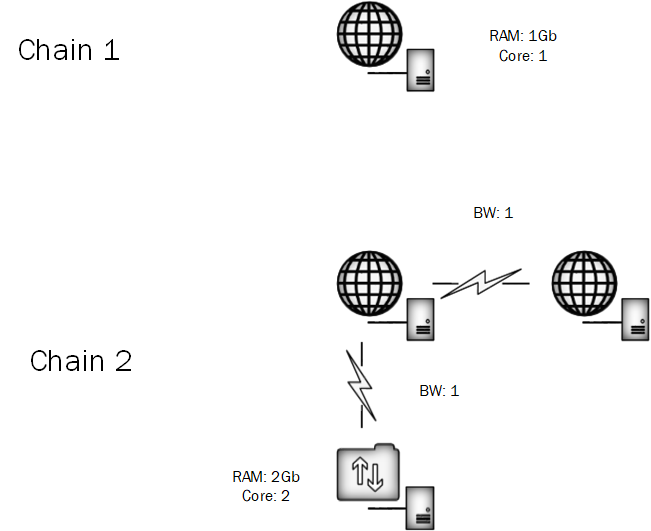
\includegraphics[scale=0.4]{../diagrams/e1-ch.png}
    \end{center}
\end{frame}
%-------------------------------------------------------------------------------
\begin{frame}{ارزیابی} % 34
    \par
    فرض می‌کنیم مرکز داده‌ای دارای توپولوژی زیر می‌باشد.

    \begin{center}
        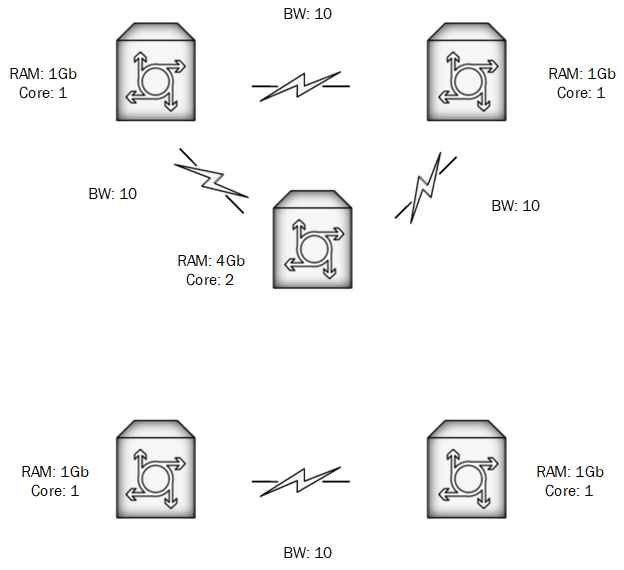
\includegraphics[scale=0.4]{../diagrams/e1-tp.png}
    \end{center}
\end{frame}
%-------------------------------------------------------------------------------
\begin{frame}[fragile]{ارزیابی} % 35
    \par
    در نهایت نتیجه زیر از مساله حاصل می‌گردد.
    \begin{latin}\begin{verbatim}
cost = 20.0

>> Chains
Chain 0 is accepted.
Chain 1 is accepted.
       
>> Instance mapping
Chain 0:
Node 0 with type 0 is mapped on 3
Chain 1:
Node 0 with type 0 is mapped on 2
Node 1 with type 0 is mapped on 1
Node 2 with type 0 is mapped on 2
    \end{verbatim}\end{latin}
\end{frame}
%-------------------------------------------------------------------------------
\begin{frame}[fragile]{ارزیابی} % 36
    \begin{latin}\begin{verbatim}
>> Manager mapping
Chain 0 manager is 4
Chain 1 manager is 0
       
>> Instance links
Chain 1 link 1 (0 - 2) is on 2-0
Chain 1 link 0 (0 - 1) is on 3-4
       
>> Management links
Chain 0 node 0 manager is on 3-4
Chain 1 node 1 manager is on 1-2
Chain 1 node 0 manager is on 2-0
Chain 1 node 1 manager is on 2-0
Chain 1 node 2 manager is on 2-0
    \end{verbatim}\end{latin}
\end{frame}
%-------------------------------------------------------------------------------
\begin{frame}[shrink=25]{مراجع} % 37
    \begin{latin}
    \printbibliography[heading=none]
    \end{latin}
\end{frame}
\end{persian}
\end{document}
